\chapter{Results}
\label{chp:results} 

\section{Results from anechoic chamber}\label{sec:anechoic_chamber}

From \autoref{sec:microinstructions} 
%=============================
% T60p Anechoic chamber MICRO
%=============================
\begin{wrapfigure}{r}{1\textwidth}
	\begin{subfigure}{1\textwidth}
	    \centering
	    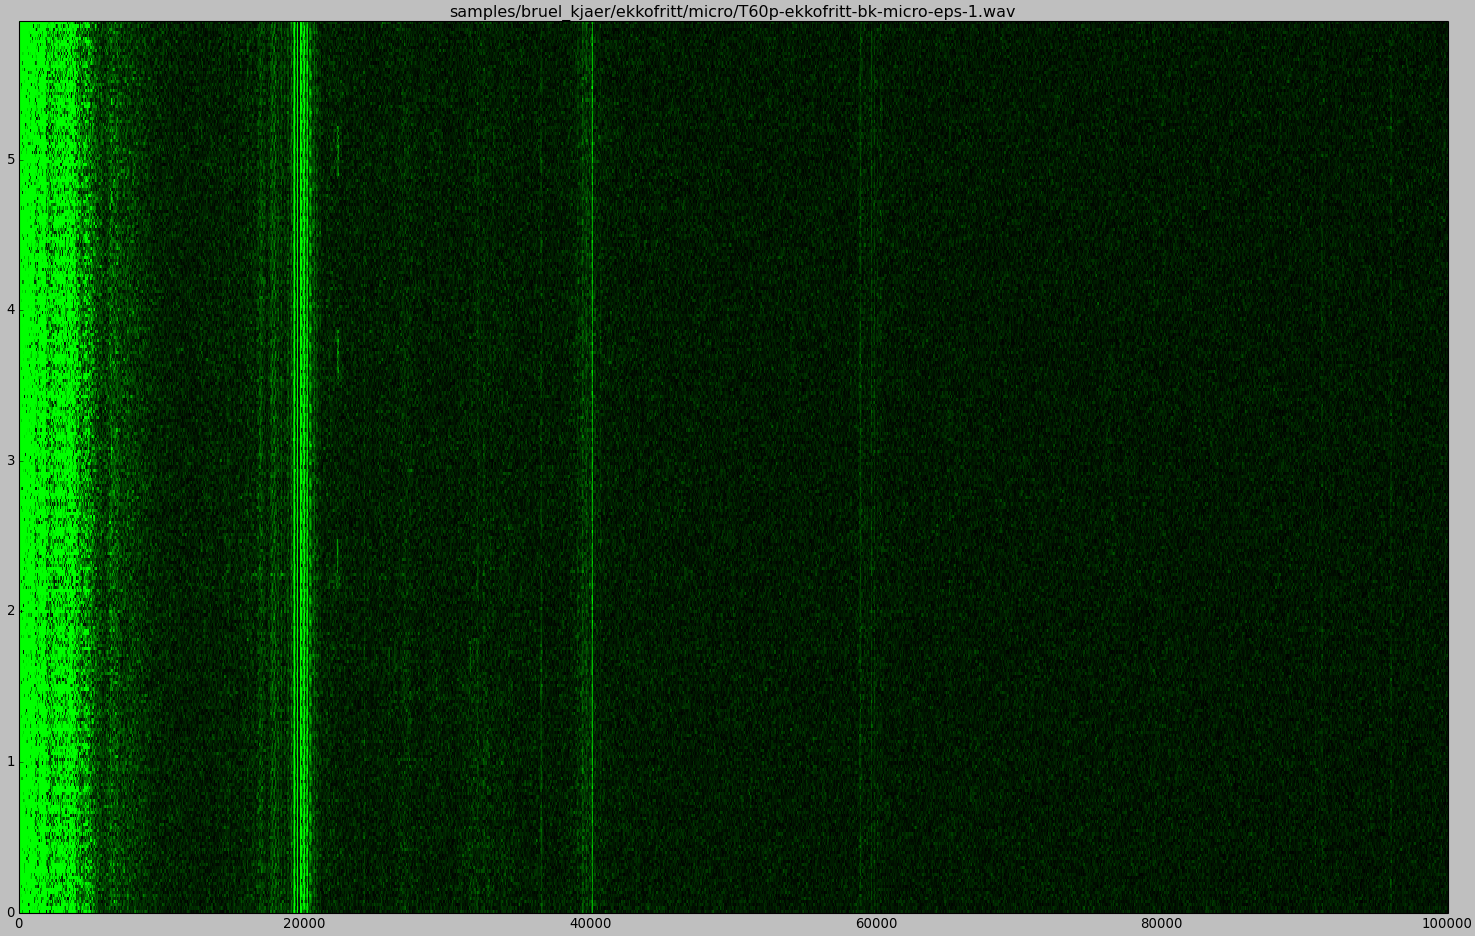
\includegraphics[width=1\linewidth]{T60p-ekkofritt-bk-micro-eps-1.png}
	    \caption{External power supply}
	    \label{fig:T60p-ekkofritt-bk-micro-eps-1}
    \end{subfigure}
    \begin{subfigure}{1\textwidth}
	    \centering
    	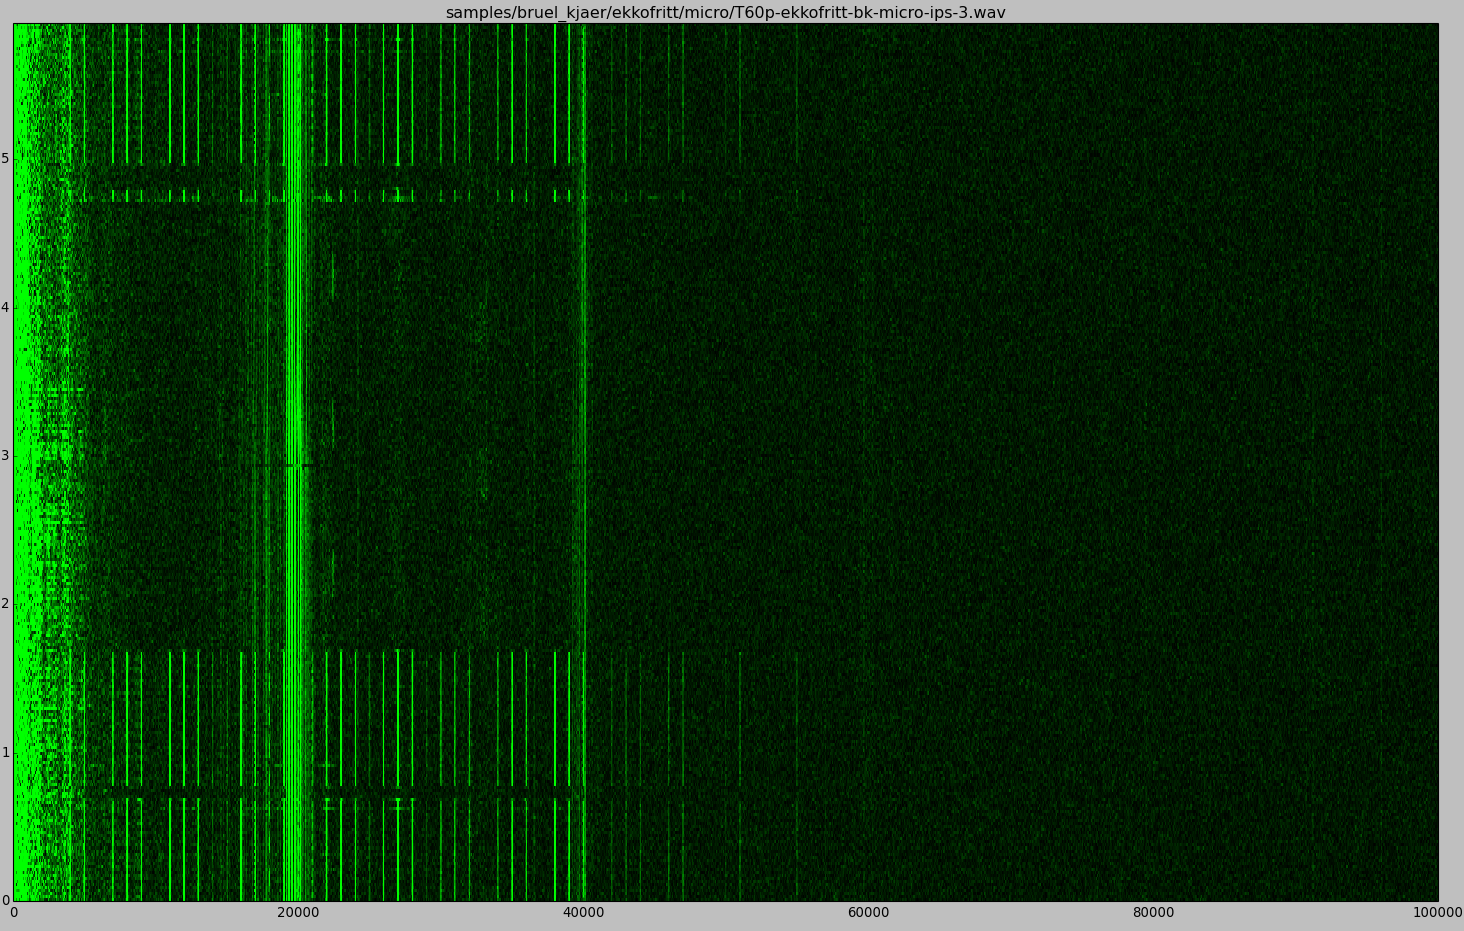
\includegraphics[width=1\linewidth]{T60p-ekkofritt-bk-micro-ips-3.png}
    	\caption{Internal power supply}
    	\label{fig:T60p-ekkofritt-bk-micro-ips-3}
    \end{subfigure}
    \caption{Acoustic recording (Vertical axis: 6 sec. Horizontal axis: 0-100kHz) of the Lenovo T60p when running microinstructions described in~\autoref{sec:microinstructions}. Both recordings was made in an anechoic chamber using the Brüel\&Kjær 4939 microphone with the NI myDAQ. }
	\label{fig:T60p-ekkofritt-bk-cpuload}
\end{wrapfigure}
%==========================
% T60p Normal room MICRO
%==========================
\begin{wrapfigure}{r}{1\textwidth}
    \centering
    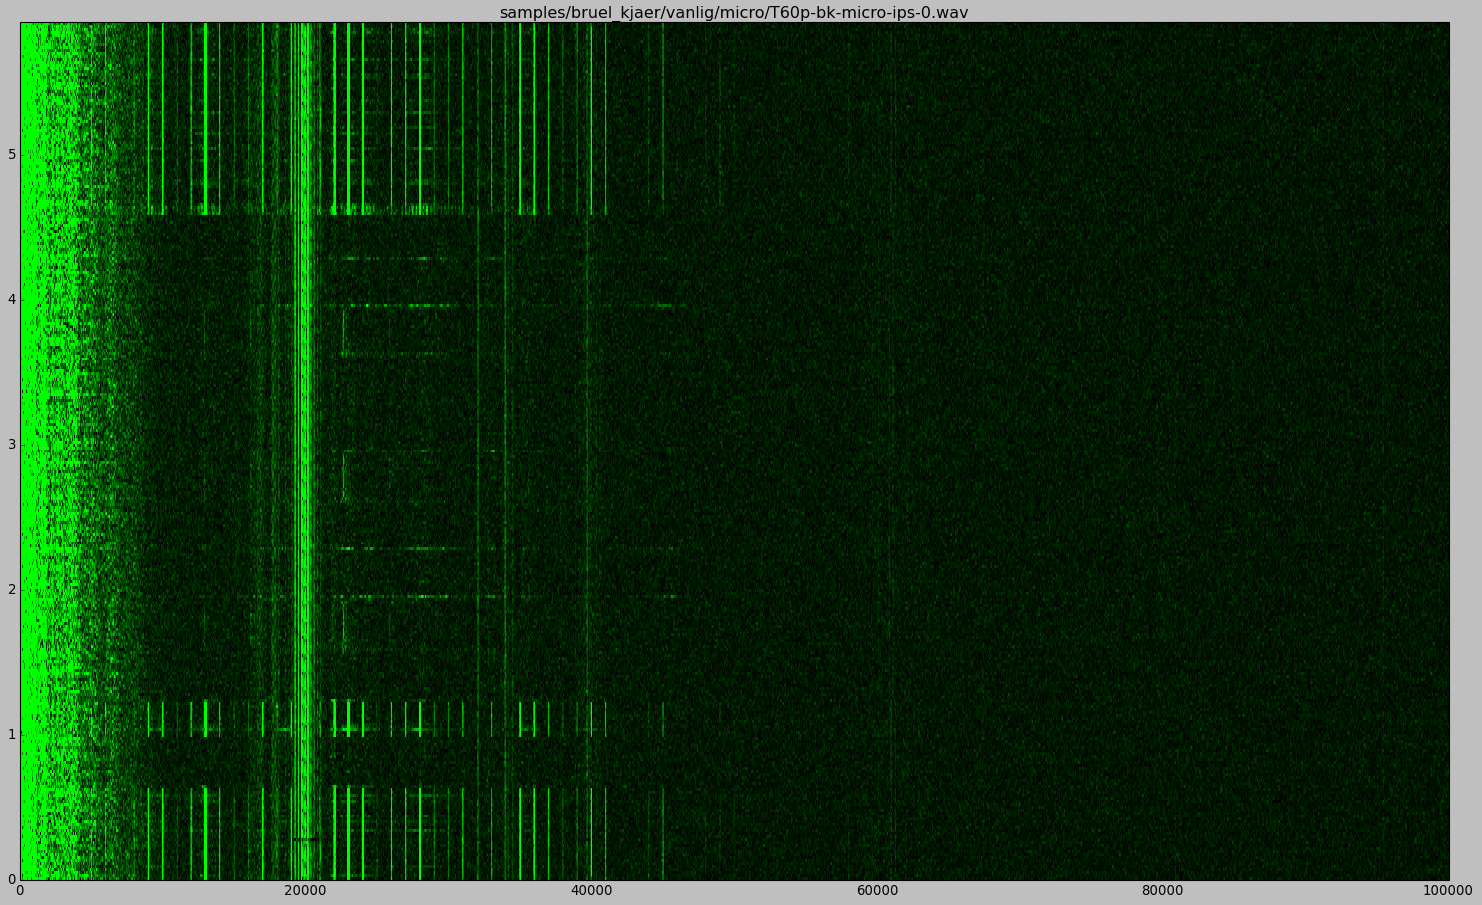
\includegraphics[width=1\linewidth]{T60p-bk-micro-ips-0.png}
    \caption{Acoustic recording (Vertical axis: 6 sec. Horizontal axis: 0-100kHz) of the Lenovo T60p when running microinstructions described in~\autoref{sec:microinstructions}. The recording was made using the Brüel\&Kjær 4939 microphone with the NI myDAQ. }
    \label{fig:T60p-bk-micro-ips-0}
\end{wrapfigure}
%===============================
% T60p Anechoic chamber CPULOAD
%===============================
\begin{wrapfigure}{r}{1\textwidth}
	\begin{subfigure}{1\textwidth}
	    \centering
	    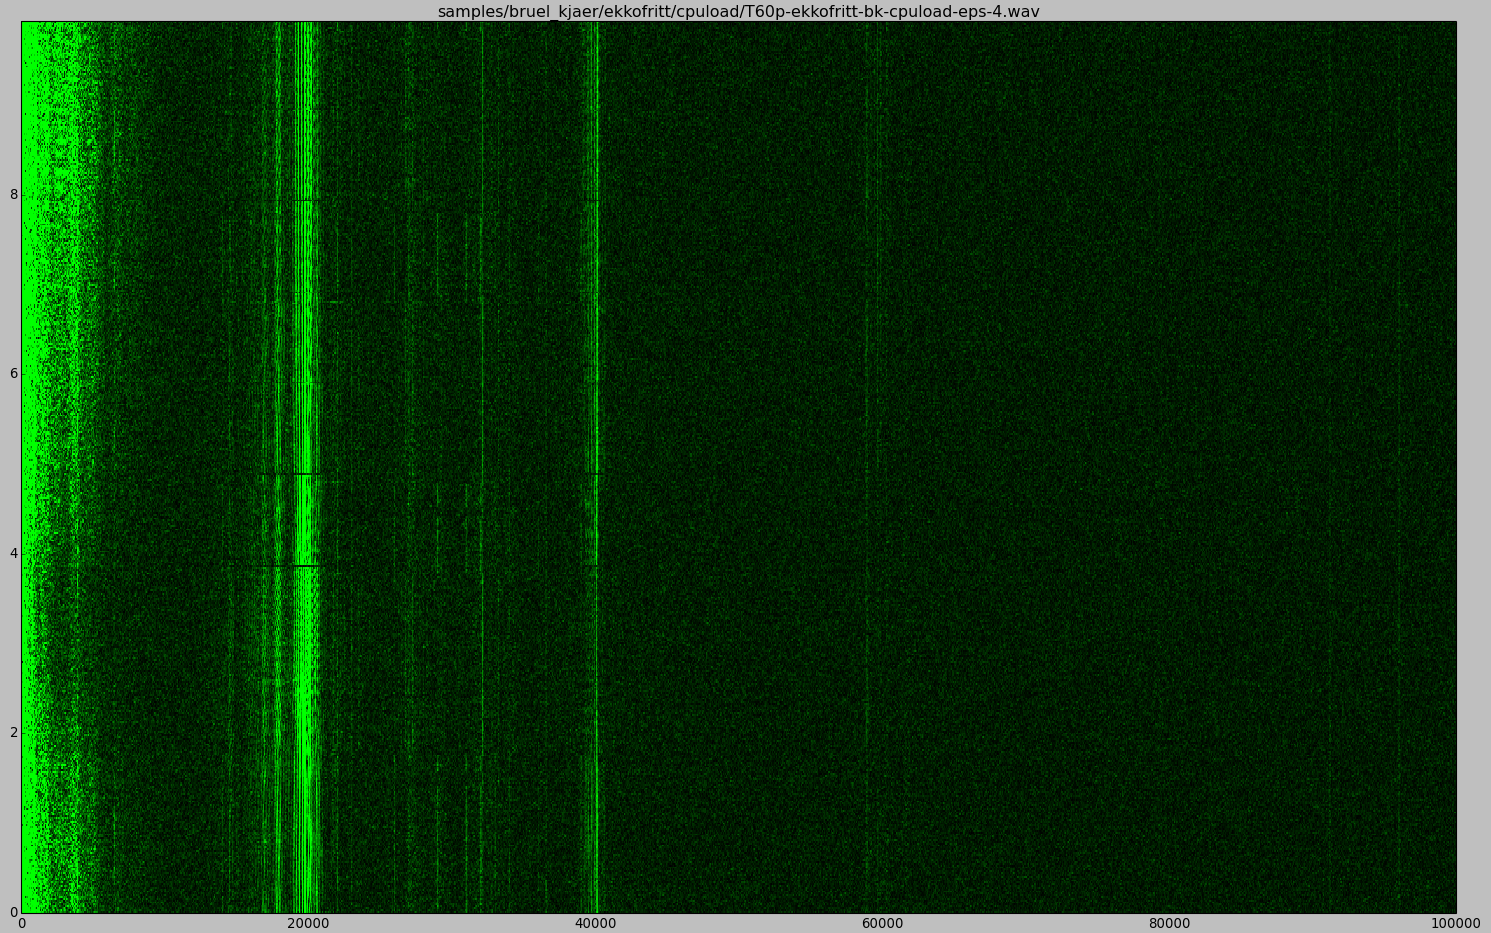
\includegraphics[width=1\linewidth]{T60p-ekkofritt-bk-cpuload-eps-4.png}
	    \caption{External power supply}
	    \label{fig:T60p-ekkofritt-bk-cpuload-eps-4}
    \end{subfigure}
    \begin{subfigure}{1\textwidth}
	    \centering
	    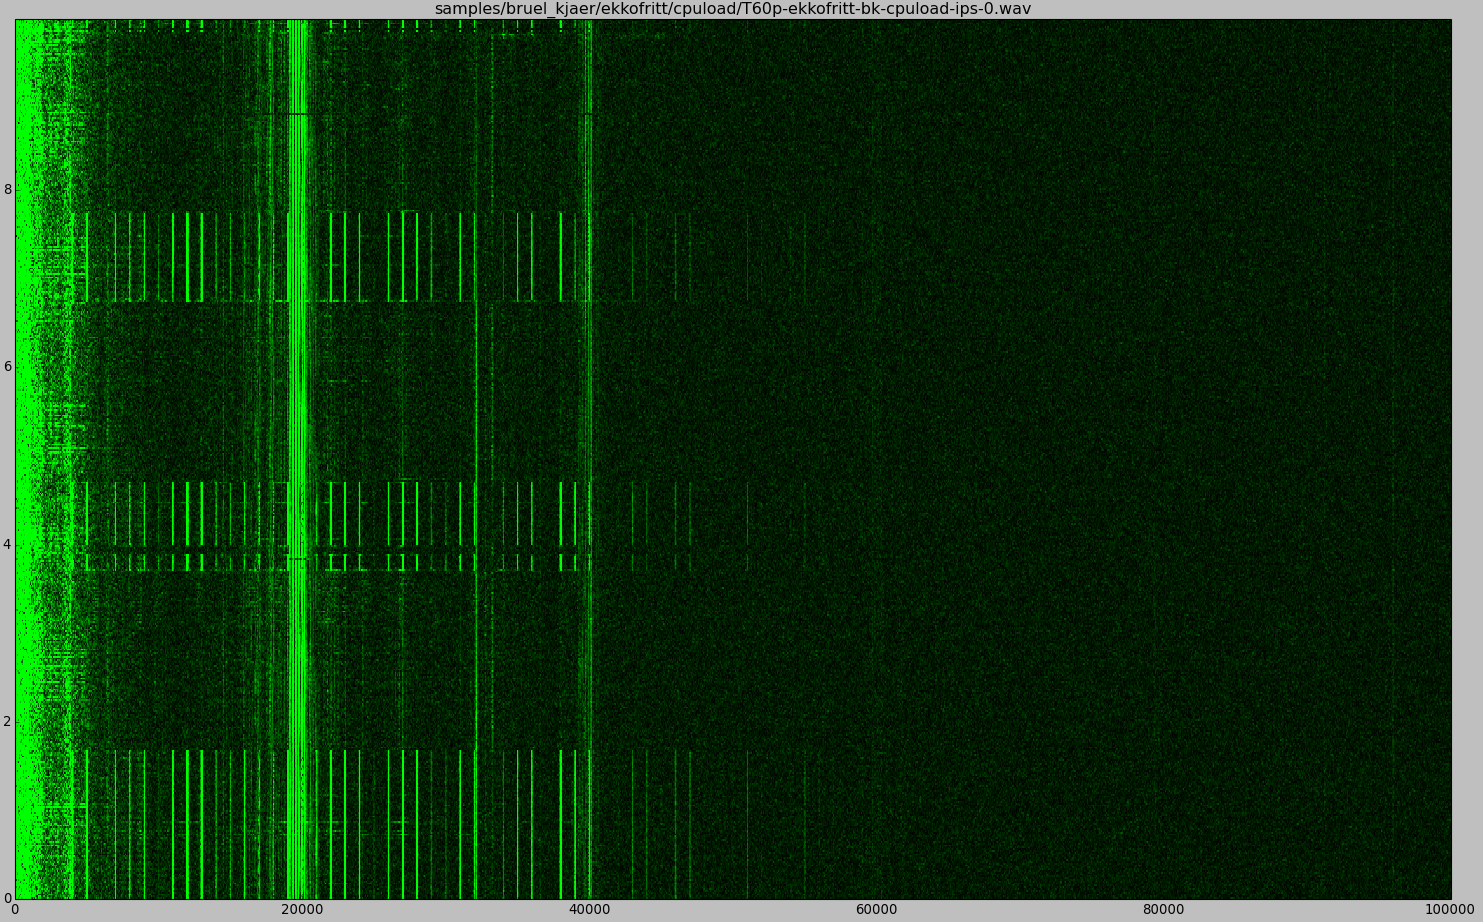
\includegraphics[width=1\linewidth]{T60p-ekkofritt-bk-cpuload-ips-0.png}
	    \caption{Internal power supply}
	    \label{fig:T60p-ekkofritt-bk-cpuload-ips-0}
    \end{subfigure}
    \caption{Acoustic recording (Vertical axis: 10 sec. Horizontal axis: 0-100kHz) of the Lenovo T60p when running a full CPU load described in~\autoref{sec:cpu-load}. The recording was made in an anechoic chamber using the Brüel\&Kjær 4939 microphone with the NI myDAQ.}
	\label{fig:T60p-ekkofritt-bk-cpuload}
\end{wrapfigure}
%==========================
% T60p Normal room CPULOAD
%==========================
\begin{wrapfigure}{r}{1\textwidth}
	\begin{subfigure}{1\textwidth}
	    \centering
	    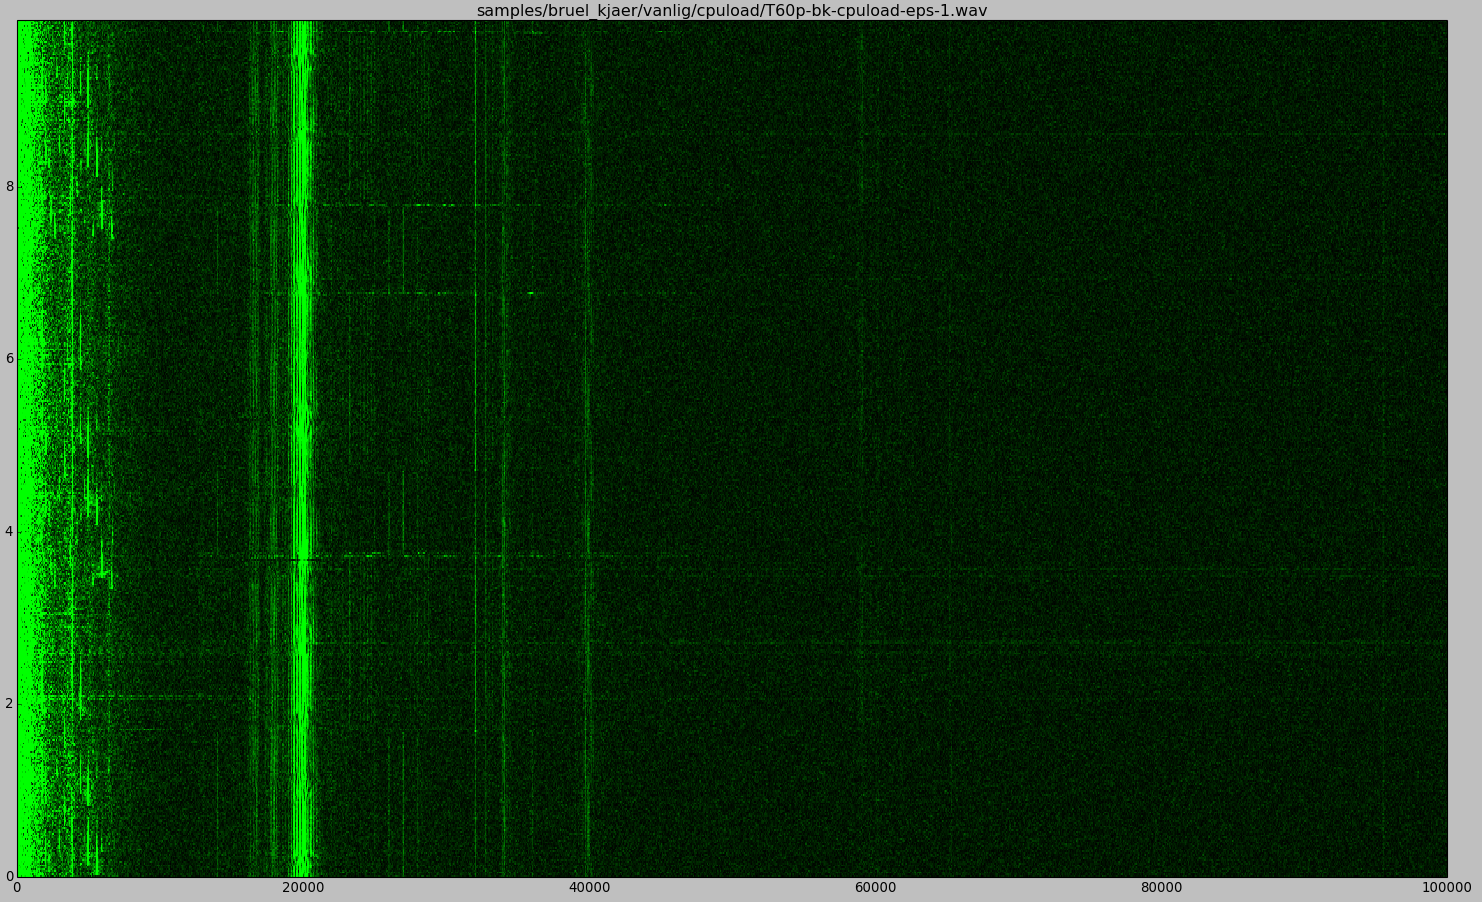
\includegraphics[width=1\linewidth]{T60p-bk-cpuload-eps-1.png}
	    \caption{External power suply}
	    \label{fig:T60p-bk-cpuload-eps-1-1a}
    \end{subfigure}
    \begin{subfigure}{1\textwidth}
	    \centering
	    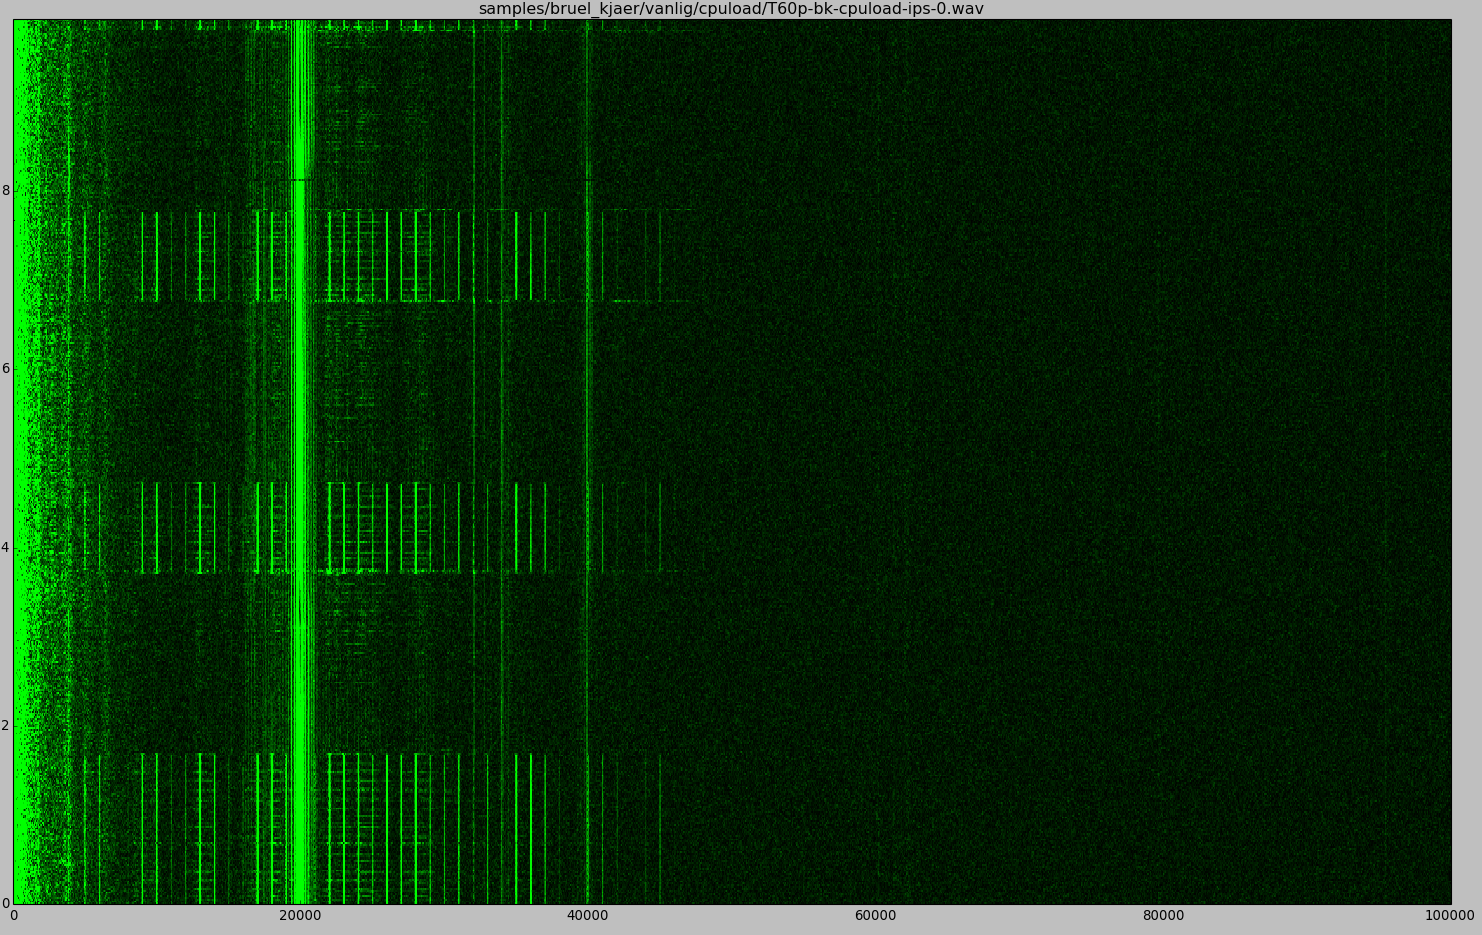
\includegraphics[width=1\linewidth]{T60p-bk-cpuload-ips-0.png}
	    \caption{Internal power suply}
	    \label{fig:T60p-bk-cpuload-ips-0-1b}
    \end{subfigure}
    \caption{Acoustic recording (Vertical axis: 10 sec. Horizontal axis: 0-100kHz) of the Lenovo T60p when running a full CPU load described in~\autoref{sec:cpu-load}. The recordings was made using the Brüel\&Kjær 4939 microphone with the NI myDAQ. }
	\label{fig:T60p-bk-cpuload}
\end{wrapfigure}
%===============================
% T60p Anechoic chamber DECRYPT
%===============================
\begin{wrapfigure}{r}{1\textwidth}
    \centering
    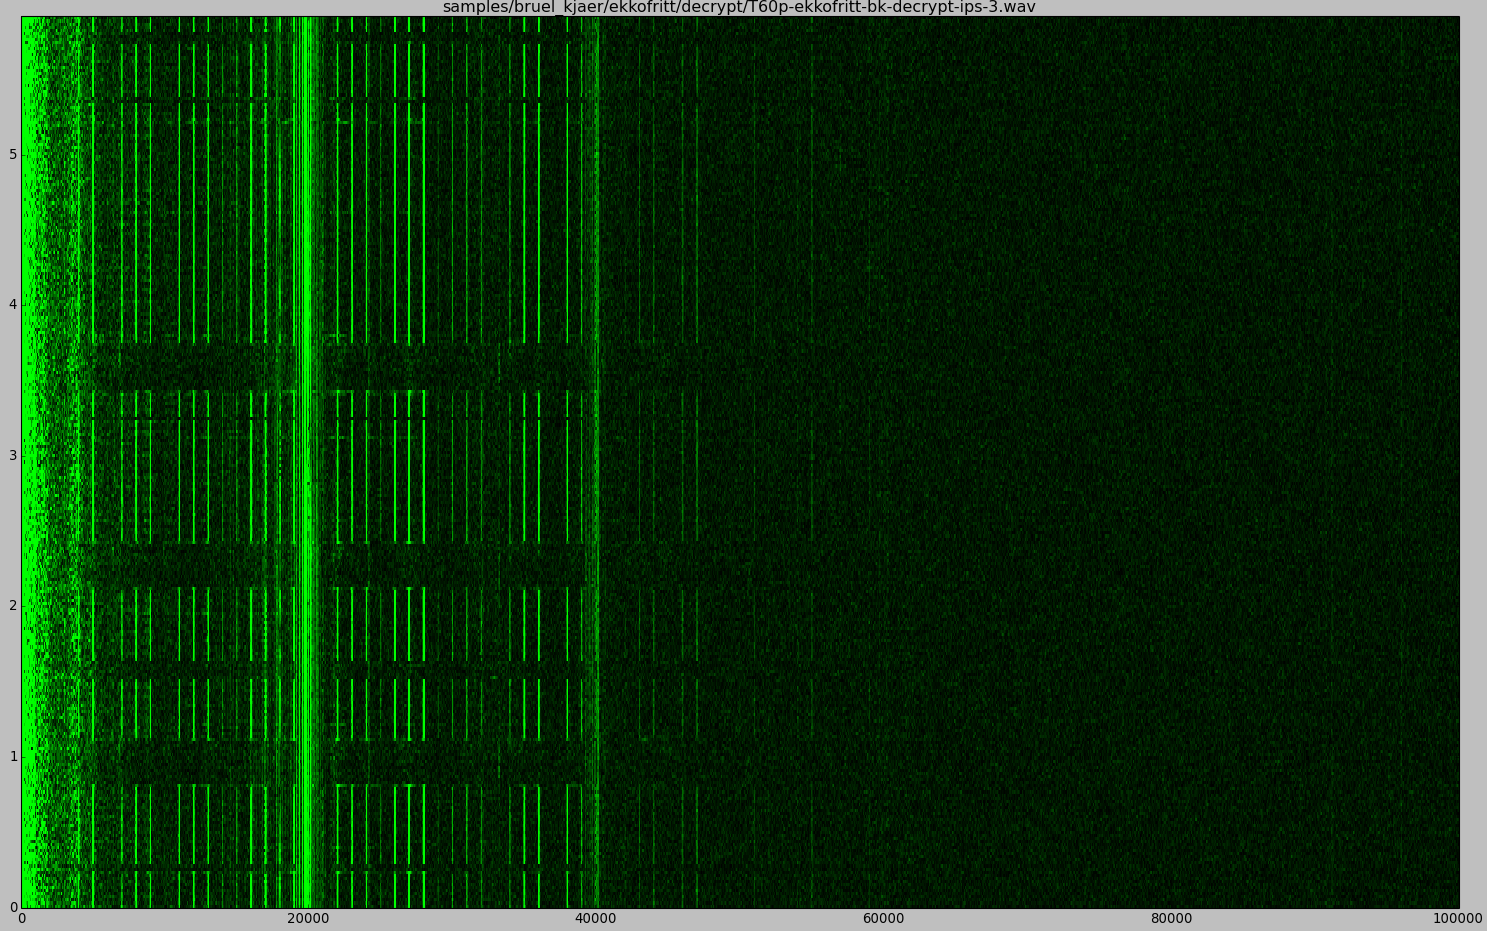
\includegraphics[width=1\linewidth]{T60p-ekkofritt-bk-decrypt-ips-3.png}
    \caption{Acoustic recording (Vertical axis: 6 sec. Horizontal axis: 0-100kHz) of the Lenovo T60p when running a decryption described in~\autoref{sec:decryption}. The recording was made in an anechoic chamber using the Brüel\&Kjær 4939 microphone with the NI myDAQ. }
    \label{fig:T60p-ekkofritt-bk-decrypt-ips-3}
\end{wrapfigure}
%================================
% D430 Anechoic chamber  CPULOAD
%================================
\begin{wrapfigure}{r}{1\textwidth}
    \centering
    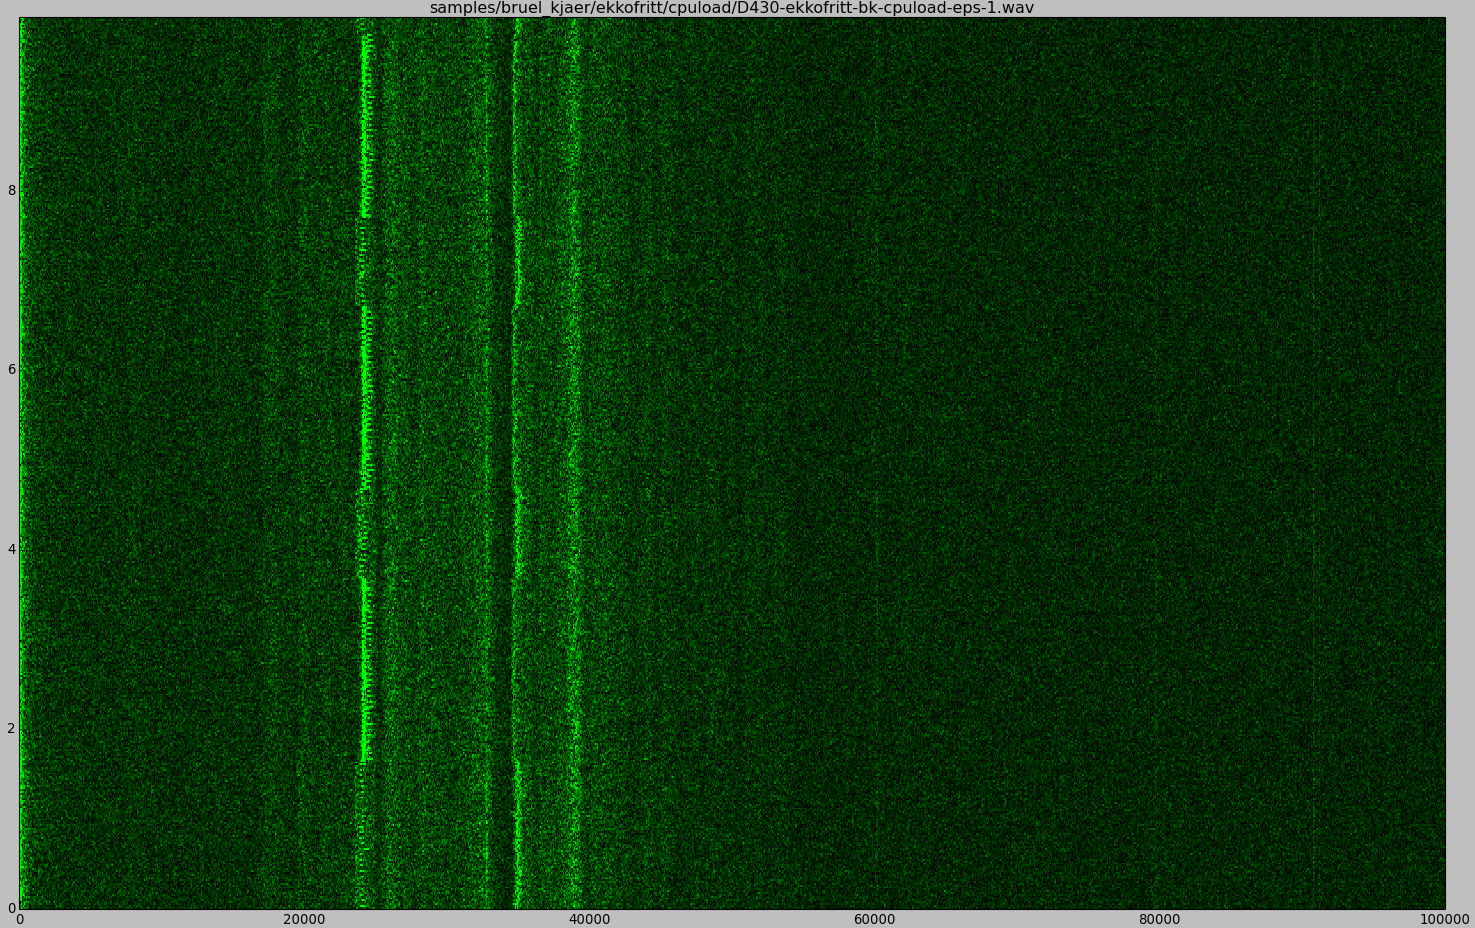
\includegraphics[width=1\linewidth]{D430-ekkofritt-bk-cpuload-eps-1.png}
    \caption{Acoustic recording (Vertical axis: 10 sec. Horizontal axis: 0-100kHz) of the Dell D430 when running a full CPU load described in~\autoref{sec:cpu-load}. The recording was made in an anechoic chamber using the Brüel\&Kjær 4939 microphone with the NI myDAQ. }
    \label{fig:D430-ekkofritt-bk-cpuload-eps-1}
\end{wrapfigure}
%================================
% D430 Anechoic chamber  DECRYPT
%================================
\begin{wrapfigure}{r}{1\textwidth}
    \centering
    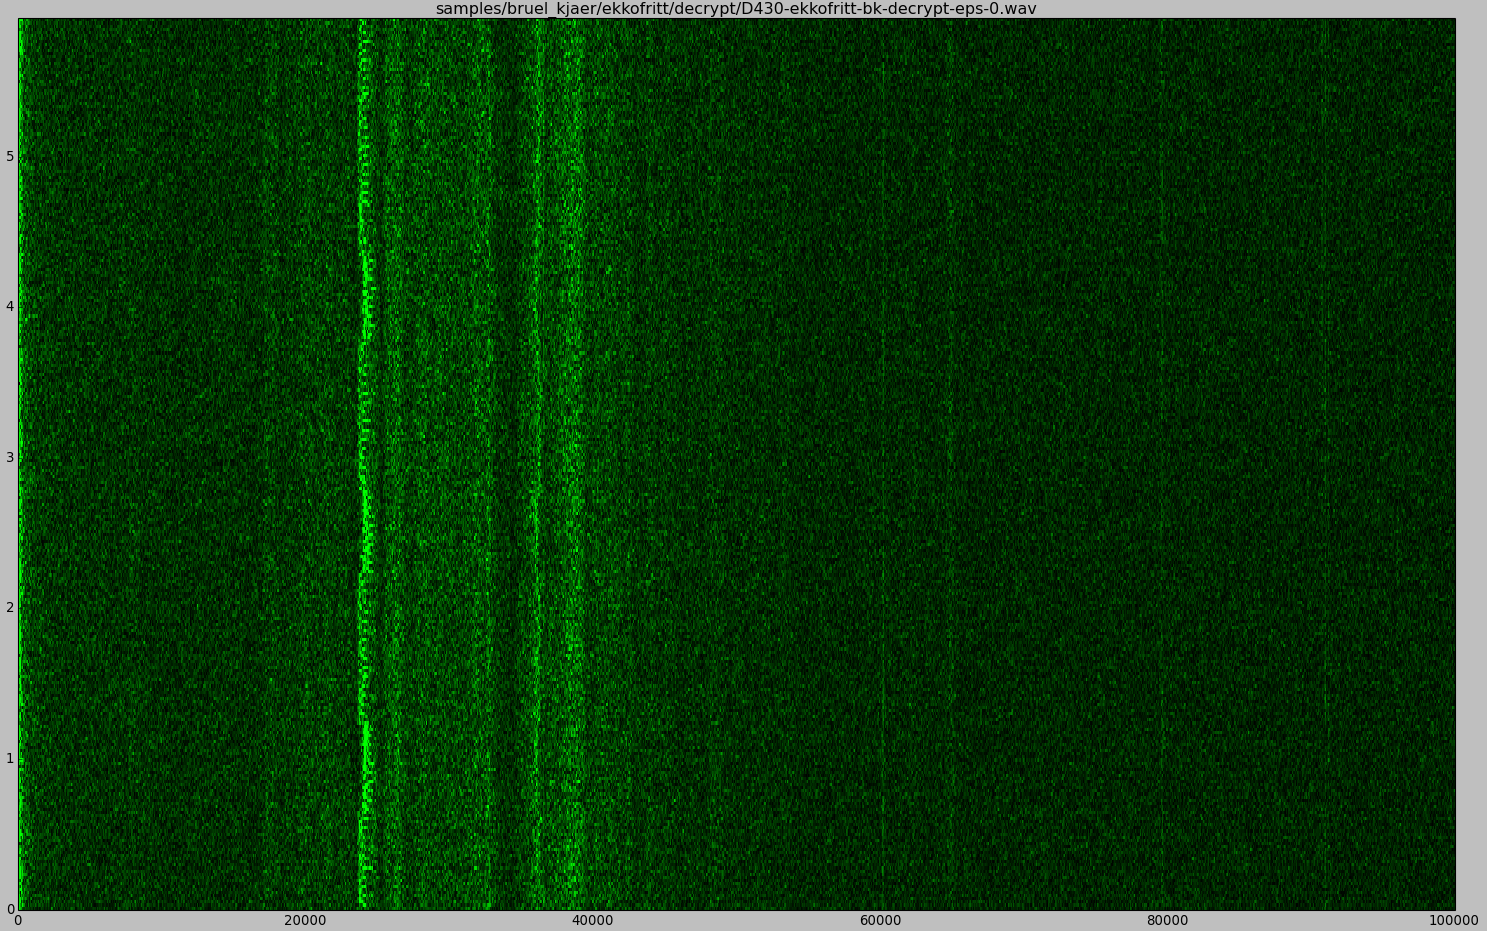
\includegraphics[width=1\linewidth]{D430-ekkofritt-bk-decrypt-eps-0.png}
    \caption{Acoustic recording (Vertical axis: 6 sec. Horizontal axis: 0-100kHz) of the Dell D430 when running a decryption described in~\autoref{sec:decryption}. The recording was made in an anechoic chamber using the Brüel\&Kjær 4939 microphone with the NI myDAQ. }
    \label{fig:D430-ekkofritt-bk-decrypt-eps-0}
\end{wrapfigure}
%=============================
% D430 Anechoic chamber  IDLE
%=============================
\begin{wrapfigure}{r}{1\textwidth}
    \centering
    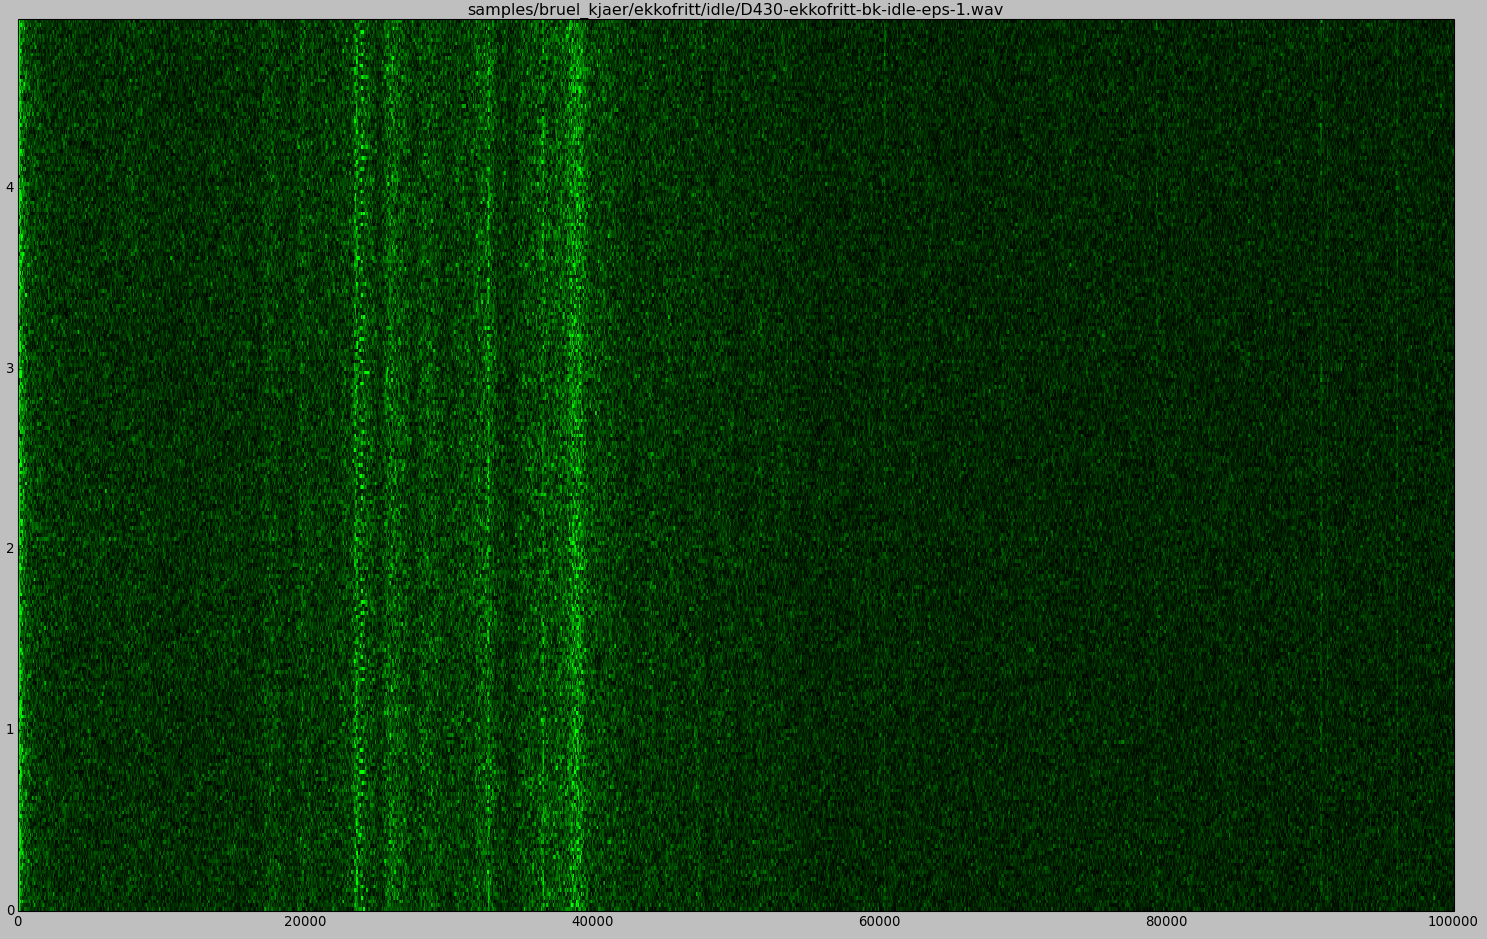
\includegraphics[width=1\linewidth]{D430-ekkofritt-bk-idle-eps-1.png}
    \caption{Acoustic recording (Vertical axis: 5 sec. Horizontal axis: 0-100kHz) of the Dell D430 when idle. The recording was made in an anechoic chamber using the Brüel\&Kjær 4939 microphone with the NI myDAQ. }
    \label{fig:D430-ekkofritt-bk-idle-eps-1}
\end{wrapfigure}